% Provenance (never printed): see sources/outline_sources.md (Year 2: interstellar
% medium, molecular clouds, gravitational collapse and the Jeans criterion, protostars
% and protostellar discs). Curves from figdata/bachelor-2/jeans.py; exercise and problem
% values in the Book 4 scratch calculator calc/ch01.py.
\chapter{अंतरतारकीय माध्यम और तारों का निर्माण}\label{ch:b2:ism-star-formation}

वृषभ तारामंडल में, सूर्य से लगभग \qty{140}{\parsec} दूर, एक काला
धब्बा अपने पीछे के तारों को ढक लेता है। कार्बन मोनोऑक्साइड की रेखाओं पर समस्वरित रेडियो दूरदर्शी से
देखने पर यह धब्बा ठंडी गैस का एक मेघ निकलता है, जो सूर्य से लगभग बीस
हज़ार गुना भारी है और तंतुओं से भरा है; उसकी सबसे सघन
गाँठों के भीतर नए तारे जन्म ले रहे हैं, और उनमें से एक, एचएल टॉरी, के चारों ओर धूल की एक
चक्रिका चमकीले और काले वलयों का एक प्रतिरूप दिखाती है, जहाँ शायद ग्रह बनने लगे
हैं। सूर्य, पृथ्वी और इस पुस्तक की चट्टानों का हर परमाणु कभी
ऐसे ही एक मेघ में था। यह अध्याय किसी ग्रहीय तंत्र के पदार्थ का अनुसरण करता है, तारों के बीच की
विरल गैस से लेकर एक नवजात तारे के चारों ओर की चक्रिका तक: \omterm{def:b2:ism-star-formation:ism}{अंतरतारकीय माध्यम} किससे
बना है, अपनी ही ऊष्मा से टिका हुआ मेघ आख़िर क्यों ढहता है,
ढहने में कितना समय लगता है, एक तारा अपना द्रव्यमान कैसे जुटाता है, और
जो पदार्थ उसमें गिरने से रह जाता है वह अंत में एक चक्रिका क्यों बनाता है।

\begin{recall}
मुख्य अनुक्रम का तारा अपने क्रोड में हाइड्रोजन को हीलियम में संलयित करके चमकता है
और अपने ही भार के विरुद्ध अपने दाब से स्वयं को थामे रखता है;
हर्ट्ज़स्प्रंग--रसेल आरेख में उसकी स्थिति उसके द्रव्यमान से तय होती है (भौतिकी,
स्नातक वर्ष 3)। द्रव्यमान $M$ के चारों ओर बंद कक्षा में घूमता पिंड केप्लर के
तीसरे नियम $T^2 = 4\pi^2 a^3/(GM)$ का पालन करता है (भौतिकी, स्नातक वर्ष 1)। तापमान $T$ की
कृष्णिका प्रति एकांक क्षेत्रफल $\sigma T^4$ उत्सर्जित करती है (भौतिकी, स्नातक
वर्ष 2)। $N$ कणों की आदर्श गैस में स्थानांतरीय गति की माध्य गतिज ऊर्जा
$\tfrac32 N k_{\mathrm B} T$ होती है। पारसेक,
\qty{3.086e16}{m}, पुस्तक 3 (स्नातक वर्ष 1) की दूरी की इकाई है।
\end{recall}

\section{तारों के बीच का पदार्थ}

तारों के बीच का आकाश ख़ाली नहीं है। सूर्य के आसपास उसमें औसतन लगभग
प्रति घन सेंटीमीटर हाइड्रोजन का एक परमाणु होता है, अर्थात् द्रव्यमान-घनत्व
\qty{2.7e-24}{g.cm^{-3}}; जिस वायु में हम साँस लेते हैं उसके उतने ही आयतन में लगभग $10^{19}$ गुना अधिक
अणु होते हैं (\cref{exo:b2:ism-star-formation:1})। पूरी आकाशगंगा में फैला यह विरल
पदार्थ फिर भी आकाशगंगीय चक्रिका के द्रव्यमान का \qtyrange{10}{15}{\percent}
है।
% ledger: ferriere:mean-density, ferriere:disc-fraction

\begin{definition}[अंतरतारकीय माध्यम, अंतरतारकीय धूल]
\label{def:b2:ism-star-formation:ism}
\emph{अंतरतारकीय माध्यम}\index{अंतरतारकीय माध्यम} वह गैस और धूल है
जो किसी आकाशगंगा के तारों के बीच के आकाश को भरती है। \emph{अंतरतारकीय
धूल}\index{अंतरतारकीय धूल} उसका वह भाग है जो ठोस कणों के रूप में है; इन कणों का आकार कुछ
नैनोमीटर से लगभग एक माइक्रोमीटर तक होता है और ये सिलिकेटों, कार्बन यौगिकों
और, ठंडे क्षेत्रों में, बर्फ़ों से बने होते हैं।
\end{definition}

इसका संघटन वही है जो सूर्य और उल्कापिंडों में मापा गया है: द्रव्यमान के अनुसार
\qty{70.4}{\percent} हाइड्रोजन, \qty{28.1}{\percent} हीलियम और
\qty{1.5}{\percent} भारी तत्त्व। द्रव्यमान का केवल \qtyrange{0.5}{1}{\percent}
धूल में है, फिर भी कुछ तत्त्वों का अधिकांश धूल में ही है: गैस में
मैग्नीशियम, सिलिकॉन और लोहा सूर्य की तुलना में 10 से 100 गुना कम हैं, क्योंकि
ये परमाणु कणों में बंद हैं, जबकि कार्बन, नाइट्रोजन और ऑक्सीजन
केवल 1.2 से 3 गुना घटे हैं। ये कण भावी ग्रहीय तंत्र के पहले ठोस हैं;
\cref{ch:b2:planet-formation-meteorites}
उनका अनुसरण करता है।
% ledger: ferriere:composition, ferriere:dust-fraction, ferriere:refractory-depletion

\subsection{पाँच प्रावस्थाएँ}

गैस एकसमान होने से बहुत दूर है। वह कुछ सुस्पष्ट अवस्थाओं, या प्रावस्थाओं, में मिलती है,
जिनमें से हर एक के तापमान और घनत्व का अपना परास है (नीचे की तालिका)। उसका लगभग आधा
द्रव्यमान उन मेघों में है जो आयतन का केवल \qtyrange{1}{2}{\percent} भरते हैं;
शेष, उष्ण या तप्त, उनके बीच का स्थान भरता है।
% ledger: ferriere:disc-fraction

\begin{table}[htbp]
\centering
\small
\begin{tabular}{lll}
\hline
प्रावस्था & तापमान (K) & घनत्व $n$ (\unit{cm^{-3}}) \\
\hline
आणविक & 10--20 & $10^2$--$10^6$ \\
शीत परमाण्विक & 50--100 & 20--50 \\
उष्ण परमाण्विक & 6000--10\,000 & 0.2--0.5 \\
उष्ण आयनित & लगभग 8000 & 0.2--0.5 \\
तप्त आयनित & लगभग $10^6$ & लगभग 0.0065 \\
\hline
\end{tabular}
\caption{सूर्य के निकट अंतरतारकीय गैस की प्रावस्थाएँ; $n$ हाइड्रोजन नाभिकों का
संख्या-घनत्व है।}
\label{tab:b2:ism-star-formation:phases}
% ledger: ferriere:molecular, ferriere:cold-atomic, ferriere:warm-atomic, ferriere:warm-ionized, ferriere:hot-ionized
\end{table}

तालिका एक नियमितता छिपाए हुए है। आदर्श गैस का दाब
$P = n k_{\mathrm B} T$ है, इसलिए गुणनफल $nT$ उसे मापता है। शीत परमाण्विक
गैस के लिए $nT$ लगभग $30\times75 \approx 2000$ है (\unit{K.cm^{-3}} में), उष्ण
परमाण्विक गैस के लिए लगभग $0.3\times8000 \approx 2400$, तप्त गैस के लिए लगभग
$0.0065\times10^6 = 6500$: कुछ गुना के अंतर के भीतर, मेघों के बीच का स्थान बाँटने वाली
तीनों प्रावस्थाएँ एक ही दाब पर हैं (नीचे का चित्र)।
जहाँ एक तप्त और एक शीत गैस बराबर दाब पर मिलती हैं, वहाँ कोई भी दूसरी को
धकेलती नहीं; स्थिर दाब पर ठंडी होती गैस उसी अनुपात में सघन होती जाती है और
उष्ण प्रावस्था से शीत प्रावस्था में आ गिरती है। \omterm{def:b2:ism-star-formation:molecular-cloud}{आणविक मेघ} कहीं ऊँचे दाबों तक पहुँचते हैं, अपने सघन भागों में हज़ारों गुना अधिक तक: वे अपने ही गुरुत्व से बँधे हैं, अपने परिवेश के
दाब से नहीं।

\begin{omfigure}
\begin{tikzpicture}
\begin{axis}[omrecord, width=0.86\linewidth, height=6.4cm, xmode=log, ymode=log,
  xmin=1e-3, xmax=1e7, ymin=3, ymax=3e6,
  xlabel={हाइड्रोजन नाभिकों का घनत्व $n$ (\unit{cm^{-3}})}, ylabel={तापमान $T$ (K)},
  tick label style={font=\scriptsize}, label style={font=\small}, clip=false,
  legend pos=north east, legend style={font=\scriptsize, draw=black!30}]
\addplot[black!45, densely dashed, domain=1e-3:1e3, samples=2] {3000/x};
\addlegendentry{$nT = \num{3000}$}
\addplot[black!60, densely dotted, thick, domain=0.1:1e5, samples=2] {3e5/x};
\addlegendentry{$nT = 3\times10^5$}
\fill[blue!45, opacity=0.6] (axis cs:1e2,10) rectangle (axis cs:1e6,20);
\fill[teal!50, opacity=0.6] (axis cs:20,50) rectangle (axis cs:50,100);
\fill[orange!55, opacity=0.6] (axis cs:0.2,6000) rectangle (axis cs:0.5,10000);
\fill[red!45, opacity=0.6] (axis cs:0.2,5714) rectangle (axis cs:0.5,11200);
\fill[violet!50, opacity=0.6] (axis cs:0.00464,7.14e5) rectangle (axis cs:0.0091,1.4e6);
\node[font=\scriptsize, anchor=south east] at (axis cs:1e6,20) {आणविक मेघ};
\node[font=\scriptsize, anchor=south west] at (axis cs:50,100) {शीत परमाण्विक};
\node[font=\scriptsize, anchor=east, align=right] at (axis cs:0.17,8000) {उष्ण परमाण्विक\\और उष्ण आयनित};
\node[font=\scriptsize, anchor=west] at (axis cs:0.011,1e6) {तप्त आयनित};
\end{axis}
\end{tikzpicture}

\par\smallskip{\small सूर्य के निकट अंतरतारकीय गैस की प्रावस्थाएँ (ऊपर की तालिका के परास;
उष्ण आयनित और तप्त प्रावस्थाएँ, जो एकल मानों के रूप में दी गई हैं, 1.4 गुना चौड़े
बक्सों के रूप में खींची गई हैं)। हर धूसर रेखा के अनुदिश दाब $nk_{\mathrm B}T$ स्थिर है:
शीत, उष्ण और तप्त प्रावस्थाएँ कुछ गुना के अंतर के भीतर लगभग एक ही दाब पर हैं,
जबकि अपने ही गुरुत्व से बँधे \omterm{def:b2:ism-star-formation:molecular-cloud}{आणविक मेघ} हज़ारों गुना तक ऊँचे दाबों तक पहुँचते हैं।
डेटा: Ferrière (2001)।}
\end{omfigure}

धूल तीन तरह से अपनी उपस्थिति दिखाती है। वह अपने पीछे के तारों का प्रकाश मंद करती है,
और लाल की अपेक्षा नीले प्रकाश को अधिक मंद करती है, जिससे उसके पार देखे गए तारे
वास्तविकता से अधिक लाल दिखते हैं। वह सुदूर अवरक्त और मिलीमीटर तरंगदैर्घ्यों पर चमकती है,
कुछ दसियों केल्विन के उस तापमान पर, जहाँ तक तारों का प्रकाश उसे गरमाता है। और
वह किसी सघन मेघ के भीतर जो कुछ भी है उसे प्रकाशिक दूरदर्शियों से छिपा लेती है; इसीलिए
तारों का निर्माण रेडियो और अवरक्त तरंगदैर्घ्यों पर प्रेक्षित किया जाता है। गैस
अपनी रेखाओं से पहचानी जाती है: परमाण्विक हाइड्रोजन \qty{21}{cm} की अपनी रेडियो रेखा से,
और आणविक हाइड्रोजन, जो ठंडी होने पर लगभग विकिरण नहीं करती, अपने साथ रहने वाले
अणुओं की रेखाओं से, जिनमें कार्बन मोनोऑक्साइड प्रमुख है।

\section{आणविक मेघ}

सबसे ठंडी और सबसे सघन प्रावस्था वह है जहाँ तारे बनते हैं।

\begin{definition}[आणविक मेघ, सघन क्रोड]
\label{def:b2:ism-star-formation:molecular-cloud}
\emph{आणविक मेघ}\index{आणविक मेघ} \omterm{def:b2:ism-star-formation:ism}{अंतरतारकीय माध्यम} का वह
क्षेत्र है जो इतना सघन और अपारदर्शी हो कि उसकी हाइड्रोजन अधिकतर
अणुओं, \ce{H2}, के रूप में रहे, और धूल उसे तारों के उस पराबैंगनी प्रकाश से बचाए
जो उन्हें तोड़ देता; उसका तापमान लगभग \qty{10}{K} से \qty{20}{K} होता है।
\emph{सघन क्रोड}\index{सघन क्रोड} किसी आणविक मेघ के भीतर एक संहत संघनन है,
जो एक पारसेक के कुछ दसवें भाग या उससे भी कम चौड़ा होता है, जिसका घनत्व
प्रति घन सेंटीमीटर $10^4$ से $10^5$ कण होता है, और जिससे एक अकेला तारा या
तारों का एक छोटा समूह बनता है।
\end{definition}

मेघ एक पदानुक्रम में संगठित होते हैं (नीचे की तालिका)। वृषभ जैसे अदीप्त मेघ में
पुंज होते हैं, और पुंजों में क्रोड; हर स्तर अपने ऊपर वाले से अधिक सघन, छोटा और अधिक
शांत है: क्रोड में गैस अधिक से अधिक एक किलोमीटर प्रति सेकंड के कुछ दसवें भाग की चाल से चलती है,
जो \qty{10}{K} की गैस में ध्वनि की चाल है। कार्बन मोनोऑक्साइड में मानचित्रित
वृषभ क्षेत्र में लगभग \num{2.4e4} सौर द्रव्यमान
गैस है; उसका केवल \qtyrange{0.3}{1.2}{\percent} ही वहाँ दिखने वाले युवा तारों में बदला है,
पिछले तीन मिलियन वर्षों में, लगभग हर एक लाख वर्ष में आठ तारों की दर से।
तारों का निर्माण धीमा और अपव्ययी है।
% ledger: bt07:clouds, bt07:clumps, bt07:cores, goldsmith:taurus-mass, goldsmith:taurus-sfe, goldsmith:taurus-distance

\begin{table}[htbp]
\centering
\small
\begin{tabular}{lccc}
\hline
 & अदीप्त मेघ & पुंज & \omterm{def:b2:ism-star-formation:molecular-cloud}{सघन क्रोड} \\
\hline
द्रव्यमान (सौर द्रव्यमान) & $10^3$--$10^4$ & 50--500 & 0.5--5 \\
आकार (pc) & 2--15 & 0.3--3 & 0.03--0.2 \\
माध्य घनत्व (\unit{cm^{-3}}) & 50--500 & $10^3$--$10^4$ & $10^4$--$10^5$ \\
गैस का तापमान (K) & लगभग 10 & 10--20 & 8--12 \\
उदाहरण & वृषभ, मस्का & --- & L1544, B68 \\
\hline
\end{tabular}
\caption{एक अदीप्त \omterm{def:b2:ism-star-formation:molecular-cloud}{आणविक मेघ} का पदानुक्रम। घनत्वों में सभी
कण गिने गए हैं। डेटा: Bergin और Tafalla (2007)।}
\label{tab:b2:ism-star-formation:hierarchy}
% ledger: bt07:clouds, bt07:clumps, bt07:cores
\end{table}

मेघ इतने ठंडे क्यों हैं? गैस बाहर निकल जाने वाले फ़ोटॉन उत्सर्जित करके ऊर्जा खोती है,
और अणु दक्ष उत्सर्जक हैं: एक संघट्ट कार्बन
मोनोऑक्साइड के अणु को ऊँचे घूर्णन-स्तर पर उठा देता है, अणु मिलीमीटर तरंगदैर्घ्य का एक फ़ोटॉन
उत्सर्जित करके वापस गिरता है, और फ़ोटॉन संघट्ट की ऊर्जा अपने साथ लेकर मेघ से
बाहर चला जाता है। भीतर पहुँचने वाले मंद तारकीय प्रकाश से गरमाई गई धूल
सुदूर अवरक्त में विकिरण करती है। ऊष्मन, जो कॉस्मिक
किरणों और धूल से छनकर आए तारकीय प्रकाश से होता है, दुर्बल है; संतुलन
लगभग \qty{10}{K} पर ठहरता है। ऐसी गैस में तापीय दाब छोटा होता है, और गुरुत्व
जीत सकता है।

\begin{omfigure}
\begin{minipage}[c]{0.44\linewidth}
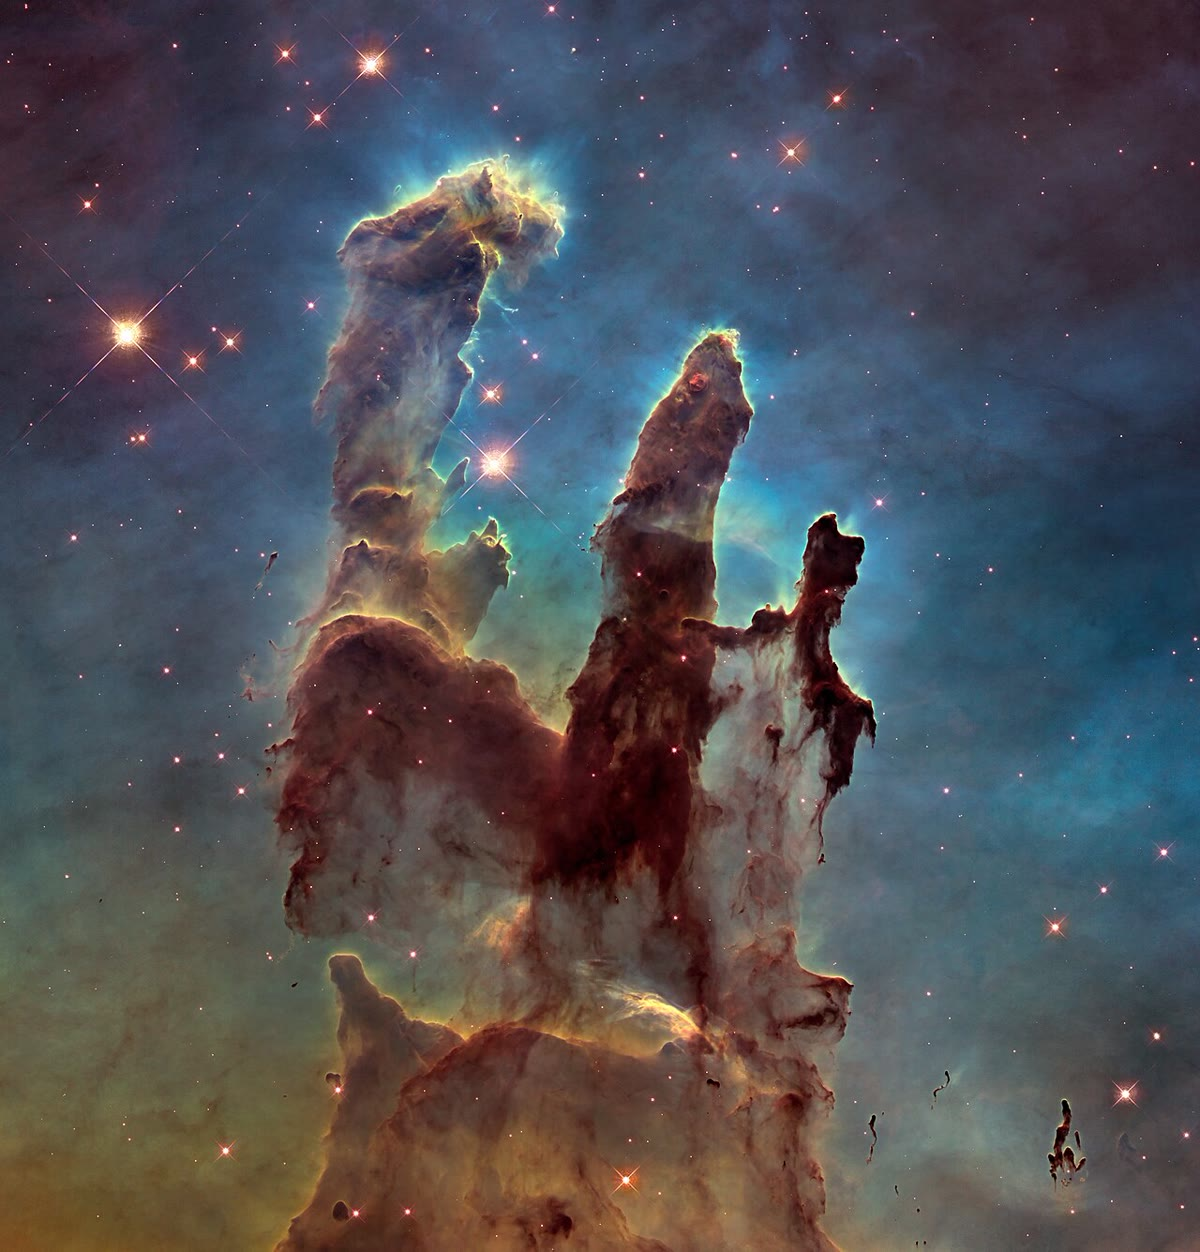
\includegraphics[width=\linewidth]{images/book4/b2-pillars-of-creation.jpg}
\end{minipage}\hfill
\begin{minipage}[c]{0.52\linewidth}
{\small ईगल नीहारिका में ``सृष्टि के स्तंभ'', हबल
अंतरिक्ष दूरदर्शी द्वारा दृश्य प्रकाश में। ये स्तंभ ठंडी, सघन आणविक गैस और
धूल हैं, प्रकाश-वर्षों लंबे, जिन्हें चित्र के बाहर के विशाल युवा तारों का पराबैंगनी प्रकाश ऊपर से
अपरदित और प्रकाशित करता है; धूल उन्हें अपारदर्शी
बनाती है। उनके सिरों पर छोटे संघनन तारे बना रहे हैं।
NASA, ESA और Hubble Heritage Team (STScI/AURA), सार्वजनिक डोमेन।}
\end{minipage}
\end{omfigure}

\section{गुरुत्वीय निपात}

मेघ दो ऊर्जाओं के बीच का संतुलन है: उसकी गैस की तापीय ऊर्जा,
जो बाहर की ओर धकेलती है, और उसकी गुरुत्वीय ऊर्जा, जो भीतर की ओर खींचती है।
दूसरी, पहली की तुलना में, द्रव्यमान के साथ तेज़ी से बढ़ती है; एक निश्चित द्रव्यमान से ऊपर गुरुत्व
जीत जाता है।

\begin{proposition}[एकसमान गोले की गुरुत्वीय ऊर्जा]
\label{prop:b2:ism-star-formation:grav-energy}
द्रव्यमान $M$ और त्रिज्या $R$ के एकसमान घनत्व वाले गोले की
गुरुत्वीय स्थितिज ऊर्जा है
\[
  U = -\frac{3}{5}\,\frac{G M^2}{R}.
\]
\end{proposition}

\begin{proof}
गोले को एक-एक कोश जोड़कर बनाइए। जब उसकी त्रिज्या $r$ हो, तब उसका द्रव्यमान
$m(r) = M r^3/R^3$ होता है; मोटाई $\mathrm dr$ और द्रव्यमान
$\mathrm dm = 3M r^2\,\mathrm dr/R^3$ के एक कोश को अनंत से उसके पृष्ठ तक लाने में
ऊर्जा $G m(r)\,\mathrm dm/r$ मुक्त होती है, क्योंकि गोला अपने बाहर ऐसे आकर्षित करता है मानो
उसका द्रव्यमान उसके केंद्र पर हो (कोश प्रमेय, भौतिकी)। अतः
\[
  U = -\int_0^R \frac{G}{r}\,\frac{M r^3}{R^3}\,\frac{3 M r^2}{R^3}\,\mathrm dr
    = -\frac{3 G M^2}{R^6}\int_0^R r^4\,\mathrm dr = -\frac{3}{5}\,\frac{G M^2}{R}.
  \qedhere
\]
\end{proof}

साम्यावस्था में स्थित स्व-गुरुत्वीय पिंड विरियल प्रमेय का पालन करता है: समय पर
औसत लेने पर, उसकी गतिज ऊर्जा का दोगुना और उसकी गुरुत्वीय ऊर्जा का योग शून्य होता है,
$2K + U = 0$ (भौतिकी, स्नातक वर्ष 3, जहाँ यह गति के समीकरणों से
व्युत्पन्न किया गया है)। विरामावस्था के मेघ के लिए $K$ उसके कणों की तापीय ऊर्जा है।
यदि $2K > |U|$ हो तो गैस फैलती है; यदि $2K < |U|$ हो तो गुरुत्व के विरोध में कोई
साम्यावस्था नहीं रहती और मेघ सिकुड़ता है।

\begin{proposition}[जीन्स कसौटी]\label{prop:b2:ism-star-formation:jeans}
तापमान $T$ और घनत्व $\rho$ का एकसमान, समतापी मेघ, जो
माध्य द्रव्यमान $\mu m_u$ के कणों से बना हो, अपने ही गुरुत्व से ढह जाता है यदि उसका द्रव्यमान
\emph{\omterm{def:b2:ism-star-formation:jeans}{जीन्स द्रव्यमान}}
\[
  M_J = \left(\frac{5 k_{\mathrm B} T}{G\mu m_u}\right)^{3/2}
        \left(\frac{3}{4\pi\rho}\right)^{1/2},
\]
से अधिक हो, या तुल्यतः यदि उसकी त्रिज्या \emph{\omterm{def:b2:ism-star-formation:jeans}{जीन्स लंबाई}}
\[
  R_J = \left(\frac{15 k_{\mathrm B} T}{4\pi G\mu m_u\,\rho}\right)^{1/2}.
\]
से अधिक हो। यही \emph{जीन्स कसौटी}\index{जीन्स कसौटी} है।
\end{proposition}

\begin{proof}
मेघ में $N = M/(\mu m_u)$ कण हैं, जिनकी तापीय ऊर्जा
$K = \tfrac32 N k_{\mathrm B}T = \tfrac32 M k_{\mathrm B}T/(\mu m_u)$ है।
\cref{prop:b2:ism-star-formation:grav-energy} से, वह ढहता है यदि
$2K < \tfrac35 GM^2/R$ हो, अर्थात्
\[
  \frac{3 M k_{\mathrm B} T}{\mu m_u} < \frac{3}{5}\,\frac{G M^2}{R}
  \iff M > \frac{5 k_{\mathrm B} T}{G \mu m_u}\, R .
\]
$R$ का विलोपन $M = \tfrac43\pi R^3\rho$, अर्थात् $R = (3M/4\pi\rho)^{1/3}$ की सहायता से कीजिए:
$M^{2/3} > \frac{5 k_{\mathrm B}T}{G\mu m_u}\,(3/4\pi\rho)^{1/3}$, और दोनों पक्षों को
घात $3/2$ तक उठाने पर $M > M_J$ मिलता है। इसके स्थान पर $M$ का विलोपन करें तो
$\tfrac43\pi R^3\rho > 5 k_{\mathrm B}T R/(G\mu m_u)$ से $R^2 > 15
k_{\mathrm B}T/(4\pi G\mu m_u\rho)$ मिलता है, अर्थात् $R > R_J$।
\end{proof}

\begin{definition}[जीन्स द्रव्यमान, जीन्स लंबाई]\label{def:b2:ism-star-formation:jeans}
दिए गए तापमान और घनत्व वाली गैस का \emph{जीन्स द्रव्यमान}\index{जीन्स द्रव्यमान} $M_J$ और \emph{जीन्स
लंबाई}\index{जीन्स लंबाई} $R_J$ वे द्रव्यमान और त्रिज्या हैं
जिनसे ऊपर उस गैस का एकसमान गोला
अपने ही गुरुत्व से ढह जाता है (\cref{prop:b2:ism-star-formation:jeans})।
\end{definition}

\omterm{def:b2:ism-star-formation:jeans}{जीन्स द्रव्यमान} $T^{3/2}$ के अनुसार बढ़ता है और $\rho^{-1/2}$ के अनुसार घटता है: ठंडी, सघन गैस
सबसे आसानी से ढहती है। \omterm{def:b2:ism-star-formation:molecular-cloud}{आणविक मेघ} में प्रति कण माध्य द्रव्यमान
$\mu = 2.33$ परमाणु द्रव्यमान मात्रक है: आणविक हाइड्रोजन, लगभग हर पाँच अणुओं पर हीलियम
के एक परमाणु के साथ। \qty{10}{K} और प्रति घन सेंटीमीटर $10^4$ कणों पर,
$\rho = \mu m_u n = \qty{3.87e-17}{kg.m^{-3}}$ और
$M_J = 5.5$ सौर द्रव्यमान, \qty{0.13}{\parsec} की \omterm{def:b2:ism-star-formation:jeans}{जीन्स लंबाई} के भीतर:
यही एक \omterm{def:b2:ism-star-formation:molecular-cloud}{सघन क्रोड} का द्रव्यमान और आकार है। अदीप्त मेघ के माध्य घनत्व,
प्रति घन सेंटीमीटर $100$ कणों, पर \omterm{def:b2:ism-star-formation:jeans}{जीन्स द्रव्यमान} दस गुना बड़ा है, 55
सौर द्रव्यमान, और वृषभ जैसे \num{24000} सौर द्रव्यमान के मेघ में
ऐसे सैकड़ों द्रव्यमान समाते हैं (नीचे का चित्र)।
% ledger: kauffmann:mu, nist:u, const:kB, const:G, sun:mass, goldsmith:taurus-mass

\begin{omfigure}
\begin{tabular}{@{}c@{\hspace{3mm}}c@{}}
\begin{tikzpicture}
\begin{axis}[omrecord, width=0.455\linewidth, height=6.0cm, xmode=log, ymode=log,
  xmin=10, xmax=1e7, ymin=0.05, ymax=1e4,
  xlabel={$n$ (\unit{cm^{-3}})}, ylabel={जीन्स द्रव्यमान (सौर द्रव्यमान)},
  tick label style={font=\scriptsize}, label style={font=\small},
  legend style={font=\scriptsize, at={(0.97,0.97)}, anchor=north east, draw=none, fill=white, fill opacity=0.85}]
\fill[blue!12] (axis cs:1e4,0.5) rectangle (axis cs:1e5,5);
\node[font=\scriptsize, blue!50!black, anchor=north east] at (axis cs:1e5,0.5) {सघन क्रोड};
\addplot[very thick, blue!70!black] table[x=n, y=MJ10] {figdata/out/bachelor-2-jeans-jeans.dat};
\addlegendentry{\qty{10}{K}}
\addplot[very thick, orange!80!black] table[x=n, y=MJ20] {figdata/out/bachelor-2-jeans-jeans.dat};
\addlegendentry{\qty{20}{K}}
\addplot[very thick, red!75!black] table[x=n, y=MJ50] {figdata/out/bachelor-2-jeans-jeans.dat};
\addlegendentry{\qty{50}{K}}
\end{axis}
\end{tikzpicture}
&
\begin{tikzpicture}
\begin{axis}[omrecord, width=0.455\linewidth, height=6.0cm, xmode=log, ymode=log,
  xmin=10, xmax=1e7, ymin=0.01, ymax=20,
  xlabel={$n$ (\unit{cm^{-3}})}, ylabel={मुक्त पतन काल (\unit{Myr})},
  tick label style={font=\scriptsize}, label style={font=\small}]
\addplot[very thick, black!70] table[x=n, y=tff_Myr] {figdata/out/bachelor-2-jeans-tff.dat};
\fill[blue!12] (axis cs:1e4,0.05) rectangle (axis cs:1e5,0.5);
\addplot[very thick, black!70] table[x=n, y=tff_Myr] {figdata/out/bachelor-2-jeans-tff.dat};
\node[font=\scriptsize, blue!50!black, anchor=north] at (axis cs:3.2e4,0.05) {क्रोड};
\end{axis}
\end{tikzpicture}
\\[2pt]
{\small (क) \omterm{def:b2:ism-star-formation:jeans}{जीन्स द्रव्यमान}} & {\small (ख) \omterm{def:b2:ism-star-formation:free-fall}{मुक्त पतन काल}}
\end{tabular}

\par\smallskip{\small (क) तीन तापमानों के लिए कणों के घनत्व के विरुद्ध \omterm{def:b2:ism-star-formation:jeans}{जीन्स द्रव्यमान}
($\mu = 2.33$)। छायांकित बक्सा प्रेक्षित सघन क्रोडों के द्रव्यमान और घनत्व
दर्शाता है: \qty{10}{K} पर उनका द्रव्यमान \omterm{def:b2:ism-star-formation:jeans}{जीन्स द्रव्यमान} के निकट है। (ख)
\cref{prop:b2:ism-star-formation:free-fall} का \omterm{def:b2:ism-star-formation:free-fall}{मुक्त पतन काल}: प्रति घन सेंटीमीटर $10^4$ कणों पर
एक मिलियन वर्ष का एक-तिहाई, $10^2$ पर दस गुना लंबा।}
\end{omfigure}

ढहना शुरू करने वाला मेघ सघन होता जाता है, और जब तक वह ठंडा रहता है उसका \omterm{def:b2:ism-star-formation:jeans}{जीन्स द्रव्यमान}
$\rho^{-1/2}$ के अनुसार घटता है; वह तब तक ठंडा रहता है जब तक संपीडन की ऊष्मा
विकिरित कर सकता है। तब मेघ के टुकड़े अपने आप अस्थिर हो जाते हैं
और अलग-अलग ढहते हैं: मेघ \emph{विखंडित} होता है। इसीलिए तारे
समूहों में बनते हैं और इसीलिए उनके द्रव्यमान उन्हें बनाने वाले मेघों की तुलना में छोटे होते
हैं। विखंडन तब रुकता है जब गैस इतनी सघन हो जाती है कि उसका विकिरण
बाहर नहीं निकल पाता: संपीडन की ऊष्मा फँस जाती है, तापमान बढ़ता है, और
\omterm{def:b2:ism-star-formation:jeans}{जीन्स द्रव्यमान} घटना बंद कर देता है।

निपात में कितना समय लगता है? यदि दाब नगण्य हो, तो मेघ का हर कोश
केंद्र की ओर मुक्त रूप से गिरता है।

\begin{proposition}[मुक्त पतन काल]\label{prop:b2:ism-star-formation:free-fall}
घनत्व $\rho$ का एकसमान गोला, जो आरंभ में विरामावस्था में और दाबरहित हो,
समय
\[
  t_{\mathrm{ff}} = \left(\frac{3\pi}{32\,G\rho}\right)^{1/2},
\]
में अपने केंद्र तक ढह जाता है, जो उसकी त्रिज्या पर निर्भर नहीं करता।
\end{proposition}

\begin{proof}
केंद्र से दूरी $R$ पर, गोले के पृष्ठ पर, विरामावस्था में स्थित एक कण पर
विचार कीजिए। उसके भीतर के कोश उससे तेज़ या उसके साथ गिरते हैं, कभी
पीछे नहीं रहते, इसलिए उसे आकर्षित करने वाला द्रव्यमान $M = \tfrac43\pi R^3\rho$ पूरे
मार्ग में वही रहता है। उसका पथ एक अपभ्रष्ट केप्लर कक्षा है: एक दीर्घवृत्त जो चपटा होकर
एक सीधा खंड बन गया है, जिसका दूर वाला सिरा $R$ पर और आकर्षण-केंद्र
दूसरे सिरे पर है, इसलिए उसका अर्ध-दीर्घ अक्ष $a = R/2$ है। दूर वाले सिरे से
केंद्र तक गिरने में आधा आवर्तकाल लगता है; केप्लर के तीसरे नियम से
\[
  t_{\mathrm{ff}} = \frac12\cdot 2\pi\sqrt{\frac{(R/2)^3}{GM}}
  = \pi\sqrt{\frac{R^3}{8\,G\cdot\frac43\pi R^3\rho}}
  = \sqrt{\frac{3\pi}{32\,G\rho}} .
\]
$R$ कट जाता है: एकसमान गोले का हर कोश एक ही
क्षण केंद्र पर पहुँचता है।
\end{proof}

\begin{definition}[मुक्त पतन काल]\label{def:b2:ism-star-formation:free-fall}
घनत्व $\rho$ वाली गैस का \emph{मुक्त पतन काल}\index{मुक्त पतन काल}
$t_{\mathrm{ff}} = (3\pi/32G\rho)^{1/2}$ है, वह समय जो उस घनत्व का एकसमान गोला
केवल अपने गुरुत्व से ढहने में लेता।
\end{definition}

प्रति घन सेंटीमीटर $10^4$ कणों वाले \omterm{def:b2:ism-star-formation:molecular-cloud}{सघन क्रोड} के लिए \omterm{def:b2:ism-star-formation:free-fall}{मुक्त पतन काल}
\qty{0.34}{Myr} है; $10^2$ वाले पूरे अदीप्त मेघ के लिए \qty{3.4}{Myr}। यदि
आकाशगंगा का हर \omterm{def:b2:ism-star-formation:molecular-cloud}{आणविक मेघ} एक \omterm{def:b2:ism-star-formation:free-fall}{मुक्त पतन काल} में ढहकर तारों में बदल जाता,
तो आकाशगंगा वास्तविकता से कहीं तेज़ी से तारे बनाती: वृषभ में पिछले तीन मिलियन वर्षों में
वास्तव में तारों में बदली गैस
मेघ का लगभग एक प्रतिशत है। मेघों को
विक्षुब्ध गतियाँ और वे चुंबकीय क्षेत्र थामे रखते हैं जिन्हें गैस का आयनित अंश अपने साथ घसीटता है,
और उनकी अधिकांश गैस ढहने से पहले ही पहले विशाल तारों की पवनों और प्रकाश से बिखर
जाती है: इसीलिए वृषभ में मापी गई दक्षता कम है।
% ledger: bt07:tff

\begin{history}[जेम्स जीन्स]
जेम्स जीन्स (1877--1946) ने 1902 में अपने ही गुरुत्व के अधीन गैस के स्थायित्व का
वह विश्लेषण प्रकाशित किया जिससे \omterm{def:b2:ism-star-formation:jeans}{जीन्स द्रव्यमान} और लंबाई निकलते हैं। उन्होंने
अनंत एकसमान गैस में घनत्व की छोटी तरंगों की वृद्धि का अध्ययन किया और
पाया कि एक क्रांतिक लंबाई से लंबी तरंगों का दाब विरोध नहीं करता,
बल्कि वे बढ़ती हैं: गैस लगभग उसी आकार के संघननों में टूट जाती है। उनकी क्रांतिक
लंबाई ऊपर पाई गई त्रिज्या से केवल एक संख्यात्मक गुणक से भिन्न है; भौतिकी,
तापीय दाब के विरुद्ध गुरुत्व, वही है।
\end{history}

\section{आद्यतारे}

क्रोड का निपात एकसमान नहीं होता। थोड़ा अधिक सघन केंद्र
पहले गिरता है; वहाँ एक छोटा, सघन, गर्म पिंड बनता है जो उस पर लगातार बरसती गैस को
निगलकर बढ़ता है।

\begin{definition}[आद्यतारा]\label{def:b2:ism-star-formation:protostar}
\emph{आद्यतारा}\index{आद्यतारा} निर्माणाधीन तारा है जो अपना अधिकांश द्रव्यमान
अब भी अपने जनक क्रोड की गैस की अभिवृद्धि से प्राप्त कर रहा है; वह
गिरती गैस द्वारा मुक्त ऊर्जा से चमकता है, नाभिकीय संलयन से नहीं।
\end{definition}

\omterm{def:b2:ism-star-formation:protostar}{आद्यतारा} कितनी तेज़ी से बढ़ता है? निपात के निकट का क्रोड लगभग एक \omterm{def:b2:ism-star-formation:jeans}{जीन्स द्रव्यमान} रखता है
और लगभग एक \omterm{def:b2:ism-star-formation:free-fall}{मुक्त पतन काल} में गिरता है, इसलिए द्रव्यमान
$M_J/t_{\mathrm{ff}}$ की कोटि की दर से पहुँचता है।

\begin{proposition}[आद्यतारे की अभिवृद्धि-दर]
\label{prop:b2:ism-star-formation:accretion}
मान लीजिए $c_s = (k_{\mathrm B}T/\mu m_u)^{1/2}$ किसी क्रोड की गैस में ध्वनि की
समतापी चाल है। \omterm{def:b2:ism-star-formation:jeans}{जीन्स द्रव्यमान} और \omterm{def:b2:ism-star-formation:free-fall}{मुक्त पतन काल} का अनुपात
घनत्व पर निर्भर नहीं करता, और
\[
  \frac{M_J}{t_{\mathrm{ff}}} \approx 10\,\frac{c_s^3}{G}:
\]
\omterm{def:b2:ism-star-formation:protostar}{आद्यतारा} $c_s^3/G$ की कोटि की दर से बढ़ता है, जो केवल उसके क्रोड के
तापमान से तय होती है।
\end{proposition}

\begin{proof}
$k_{\mathrm B}T/(\mu m_u) = c_s^2$ लेने पर $M_J = 5^{3/2}\,c_s^3\,G^{-3/2}
(3/4\pi\rho)^{1/2}$ और $t_{\mathrm{ff}} = (3\pi/32)^{1/2}(G\rho)^{-1/2}$, इसलिए
\[
  \frac{M_J}{t_{\mathrm{ff}}} = 5^{3/2}\left(\frac{3}{4\pi}\right)^{1/2}
  \left(\frac{32}{3\pi}\right)^{1/2}\frac{c_s^3}{G}
  = 11.18\times0.489\times1.84\,\frac{c_s^3}{G} \approx 10\,\frac{c_s^3}{G},
\]
जिसमें $\rho$ कट गया है। गुणक क्रोड की आकृति पर निर्भर करता है;
जिन क्रोडों का घनत्व, प्रेक्षणों के अनुरूप, बाहर की ओर घटता है उनके मॉडल
स्वयं $c_s^3/G$ के अधिक निकट दरें देते हैं।
\end{proof}

\qty{10}{K} पर $c_s = \qty{0.19}{km.s^{-1}}$ और $c_s^3/G$
प्रति वर्ष \num{1.6e-6} सौर द्रव्यमान है: सूर्य जैसा तारा लगभग
\num{600000} वर्षों में जुटता है, जो उसके क्रोड के \omterm{def:b2:ism-star-formation:free-fall}{मुक्त पतन काल} के तुल्य समय है।
अधिक गर्म क्रोड में, \qty{20}{K} पर, दर $2^{3/2} = 2.8$ गुना अधिक है।

\begin{omfigure}
\begin{tikzpicture}[font=\scriptsize]
% panel 1: core
\begin{scope}
\shade[inner color=gray!70, outer color=gray!10] (0,0) circle (1.0);
\node[align=center] at (0,-1.45) {(1) सघन क्रोड\\$\sim\qty{0.1}{pc}$, \qty{10}{K}};
\end{scope}
% panel 2: collapse with infall arrows
\begin{scope}[xshift=3.0cm]
\shade[inner color=gray!80, outer color=gray!10] (0,0) circle (0.9);
\foreach \a in {0,45,...,315} \draw[-{Stealth[length=1.6mm]}, black!70] (\a:0.85) -- (\a:0.3);
\fill[orange!90!red] (0,0) circle (0.07);
\node[align=center] at (0,-1.45) {(2) निपात\\$t_{\mathrm{ff}} \sim \qty{0.1}{Myr}$};
\end{scope}
% panel 3: protostar with disc and outflow
\begin{scope}[xshift=6.0cm]
\fill[gray!25] (0,0) ellipse (0.9 and 0.6);
\fill[brown!55] (0,0) ellipse (0.75 and 0.12);
\fill[orange!90!red] (0,0) circle (0.08);
\fill[blue!25] (0,0.1) -- (-0.22,0.95) -- (0.22,0.95) -- cycle;
\fill[blue!25] (0,-0.1) -- (-0.22,-0.95) -- (0.22,-0.95) -- cycle;
\node[align=center] at (0,-1.45) {(3) आद्यतारा, चक्रिका\\और बहिर्प्रवाह, $\sim\qty{0.5}{Myr}$};
\end{scope}
% panel 4: T Tauri with disc
\begin{scope}[xshift=9.0cm]
\fill[brown!55] (0,0) ellipse (0.85 and 0.1);
\fill[yellow!80!orange] (0,0) circle (0.1);
\draw[blue!40, thick] (0,0.15) -- (0,0.6); \draw[blue!40, thick] (0,-0.15) -- (0,-0.6);
\node[align=center] at (0,-1.45) {(4) टी टॉरी तारा\\और चक्रिका, 1--\qty{5}{Myr}};
\end{scope}
% panel 5: planetary system
\begin{scope}[xshift=12.0cm]
\fill[yellow!80!orange] (0,0) circle (0.12);
\foreach \r in {0.3,0.5,0.8} \draw[black!40] (0,0) ellipse ({\r} and {0.4*\r});
\fill (0.3,0) circle (0.03); \fill (-0.5,0.03) circle (0.035); \fill (0.8,0.05) circle (0.06);
\node[align=center] at (0,-1.45) {(5) मुख्य अनुक्रम का\\तारा और ग्रह};
\end{scope}
\foreach \x in {1.4,4.4,7.4,10.4} \draw[-{Stealth}, thick, black!60] (\x,0) -- (\x+0.25,0);
\end{tikzpicture}

\par\smallskip{\small \omterm{def:b2:ism-star-formation:molecular-cloud}{सघन क्रोड} से ग्रहीय तंत्र तक (व्यवस्था-चित्र, पैमाने पर नहीं)।
(1) \omterm{def:b2:ism-star-formation:jeans}{जीन्स द्रव्यमान} के निकट एक ठंडा क्रोड। (2) उसका केंद्र पहले ढहता है और एक \omterm{def:b2:ism-star-formation:protostar}{आद्यतारा}
बनता है। (3) \omterm{def:b2:ism-star-formation:protostar}{आद्यतारा} एक चक्रिका के माध्यम से अभिवृद्धि द्वारा बढ़ता है, जबकि एक \omterm{def:b2:ism-star-formation:t-tauri}{द्विध्रुवी बहिर्प्रवाह}
घूर्णन-अक्ष के अनुदिश गैस को साफ़ करता है। (4) आवरण के समाप्त होने पर, एक \omterm{def:b2:ism-star-formation:t-tauri}{टी टॉरी तारा}, जो अब भी
सिकुड़ रहा है, अपनी चक्रिका से घिरा रहता है। (5) चक्रिका बिखर चुकी है; उसके ठोसों में से
जो बचा है वह ग्रह हैं। समय पाठ के मुक्त पतन और अभिवृद्धि के आकलनों से
और अंतिम अनुभाग की चक्रिका-आयुओं से लिए गए हैं।}
\end{omfigure}

जब तक अभिवृद्धि चलती है, \omterm{def:b2:ism-star-formation:protostar}{आद्यतारा} गिरती गैस की ऊर्जा से चमकता है। जब
आवरण चुक जाता है, तब भी वह, अब भी बिना संलयन के,
सिकुड़कर चमकता रहता है।

\begin{proposition}[संकुचन युवा तारे को ऊर्जा देता है]
\label{prop:b2:ism-star-formation:contraction}
साम्यावस्था में स्थित स्व-गुरुत्वीय गैस-गोला जो धीरे-धीरे सिकुड़ता है, वह जितनी गुरुत्वीय ऊर्जा
मुक्त करता है उसका आधा विकिरित करता है और शेष आधा ऊष्मा के रूप में रखता है:
ऊर्जा खोते हुए भी वह अधिक गर्म होता जाता है।
\end{proposition}

\begin{proof}
साम्यावस्था में विरियल प्रमेय से $2K + U = 0$ मिलता है, इसलिए कुल ऊर्जा
$E = K + U = U/2$ है। यदि त्रिज्या घटे, तो $U$ किसी राशि
$\Delta < 0$ से घटता है; तब $E$ में $\Delta/2$ का परिवर्तन होता है, जो विकिरित होकर निकली
ऊर्जा है, और $K = -U/2$ में $-\Delta/2 > 0$ का परिवर्तन होता है: तापीय ऊर्जा, और इसलिए
तापमान, शेष आधे से बढ़ते हैं।
\end{proof}

\begin{definition}[केल्विन--हेल्महोल्ट्ज़ काल-मान]\label{def:b2:ism-star-formation:kh-time}
द्रव्यमान $M$, त्रिज्या $R$ और ज्योति $L$ वाले तारे का
\emph{केल्विन--हेल्महोल्ट्ज़ काल-मान}\index{केल्विन--हेल्महोल्ट्ज़ काल-मान}
$t_{\mathrm{KH}} = GM^2/(RL)$ है, अर्थात् उस समय की परिमाण की कोटि जितने समय तक
केवल संकुचन उसकी ज्योति की पूर्ति कर सकता है।
\end{definition}

वर्तमान सूर्य के लिए $t_{\mathrm{KH}} = \qty{31}{Myr}$ है: उसकी आयु से बहुत
कम, इसीलिए सूर्य को हाइड्रोजन जलानी ही पड़ती है। एक सौर द्रव्यमान के युवा तारे के लिए,
जिसकी त्रिज्या और ज्योति सूर्य की दोगुनी हों, यह \qty{8}{Myr} है
(\cref{exo:b2:ism-star-formation:6})। संकुचन तब समाप्त होता है जब केंद्र इतना गर्म हो जाता है कि हाइड्रोजन-संलयन
ज्योति की पूर्ति कर सके: तारा मुख्य अनुक्रम पर पहुँच जाता है (पहले से ज्ञात)।
% ledger: sun:mass, sun:R, sun:L, const:G

\begin{definition}[टी टॉरी तारा, द्विध्रुवी बहिर्प्रवाह]\label{def:b2:ism-star-formation:t-tauri}
\emph{टी टॉरी तारा}\index{टी टॉरी तारा} लगभग दो सौर द्रव्यमान से कम का युवा तारा है
जिसने अपना आवरण उतार दिया है और दिखने लगा है, पर जो अभी
मुख्य अनुक्रम तक नहीं पहुँचा है: वह संकुचन से चमकता है, उसकी चमक
बदलती रहती है, और वह प्रायः एक चक्रिका से घिरा रहता है जिससे वह अब भी
अभिवृद्धि करता है। \emph{द्विध्रुवी बहिर्प्रवाह}\index{द्विध्रुवी बहिर्प्रवाह} गैस के तीव्र
जेटों या पवनों का वह युग्म है जिसे युवा तारा अपनी चक्रिका के घूर्णन-अक्ष के अनुदिश
विपरीत दिशाओं में फेंकता है।
\end{definition}

बहिर्प्रवाह उस गैस के कोणीय संवेग का एक भाग ले जाते हैं जिसे चक्रिका तारे तक
पहुँचाती है, और अक्ष के अनुदिश आवरण को साफ़ करते हैं; एचएल टॉरी का
तारा, अपनी आद्यतारकीय अवस्था के अंत में, एक अत्यधिक संरेखित बहिर्प्रवाह
चलाता है।
% ledger: alma:hltau

\section{चक्रिकाएँ}

\omterm{def:b2:ism-star-formation:molecular-cloud}{सघन क्रोड} धीरे-धीरे घूमता है: एक क्रोड के आर-पार गैस का वेग प्रति पारसेक एक किलोमीटर
प्रति सेकंड के कुछ दसवें भाग बदलता है। जैसे-जैसे क्रोड ढहता है, उसका
कोणीय संवेग संरक्षित रहता है, और धीमा घूर्णन तेज़ हो जाता है।

\begin{proposition}[अपकेंद्री त्रिज्या]\label{prop:b2:ism-star-formation:centrifugal}
विशिष्ट कोणीय संवेग $j$ (प्रति एकांक द्रव्यमान कोणीय संवेग) वाली गैस
जो द्रव्यमान $M$ की ओर गिर रही हो, केंद्र तक नहीं पहुँच सकती: वह एक वृत्तीय
कक्षा पर ठहर जाती है, जिसकी त्रिज्या है
\[
  r_c = \frac{j^2}{G M}.
\]
\end{proposition}

\begin{proof}
घर्षण के बिना गिरती गैस का कोणीय संवेग संरक्षित रहता है, इसलिए
दूरी $r$ पर उसकी घूर्णन-चाल $v = j/r$ होती है। गैस $r$ पर तभी परिक्रमा कर सकती है जब
गुरुत्व ठीक-ठीक अभिकेंद्र त्वरण प्रदान करे,
$GM/r^2 = v^2/r = j^2/r^3$, अर्थात् $r = j^2/(GM)$ पर। इससे भीतर,
आवश्यक अभिकेंद्र त्वरण $j^2/r^3$ गुरुत्व के खिंचाव से अधिक हो जाता है, और
गैस आगे नहीं जा सकती।
\end{proof}

घूर्णन-अक्ष के अनुदिश गिरने वाली गैस में कोणीय संवेग कम होता है और वह
सीधे तारे पर जाती है; विषुवतीय तल में गिरने वाली गैस अपना
घूर्णन बनाए रखती है। विपरीत दिशाओं से भिन्न पथों पर गिरती गैस
विषुवतीय तल के ऊपर और नीचे टकराती है, अपनी ऊर्ध्वाधर गति खो देती है, और
लगभग $r_c$ त्रिज्या की एक पतली घूर्णी चक्रिका में एकत्र हो जाती है।
\qty{0.1}{pc} के एक क्रोड के लिए, जो लगभग बीस मिलियन वर्षों में एक चक्कर लगाता है, $r_c$ कुछ
सौ खगोलीय इकाई है (\cref{exo:b2:ism-star-formation:11}): प्रेक्षित चक्रिकाओं का आकार।

\begin{definition}[आद्यग्रहीय चक्रिका]\label{def:b2:ism-star-formation:disc}
\emph{आद्यग्रहीय चक्रिका}\index{आद्यग्रहीय चक्रिका} (या
\emph{आद्यतारकीय चक्रिका}\index{आद्यतारकीय चक्रिका}) युवा तारे के चारों ओर लगभग केप्लरीय
घूर्णन करती गैस और धूल की वह चपटी चक्रिका है जो उसके जनक क्रोड के उस
पदार्थ से बनी है जिसने तारे पर गिरने के लिए बहुत अधिक कोणीय संवेग बनाए रखा;
इसी में ग्रह बनते हैं।
\end{definition}

\begin{omfigure}
\begin{minipage}[c]{0.44\linewidth}
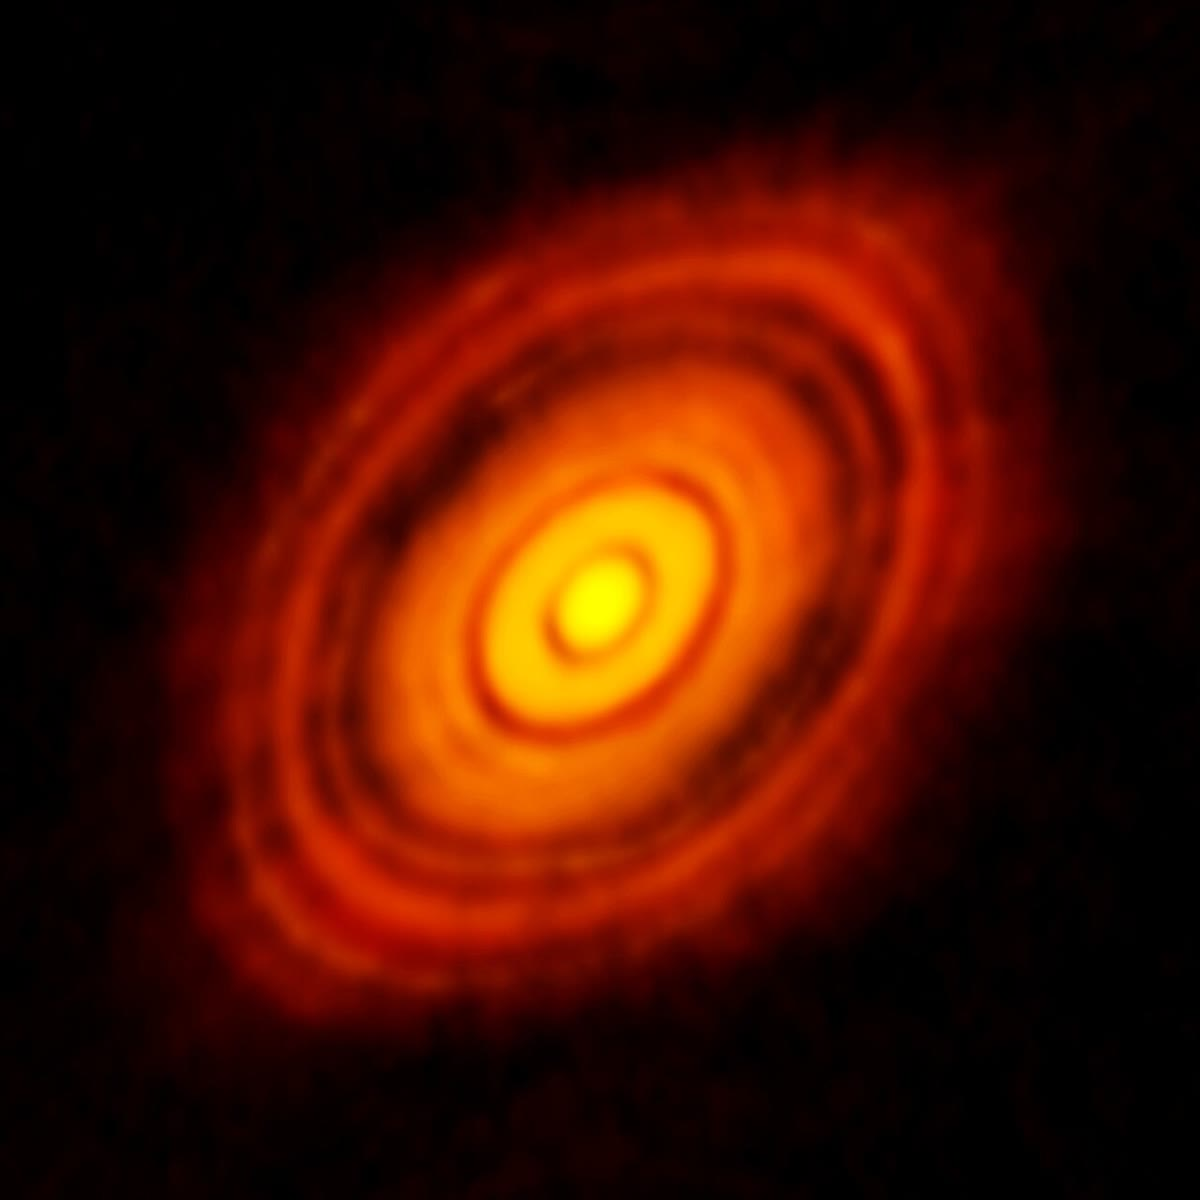
\includegraphics[width=\linewidth]{images/book4/b2-hl-tau-alma.jpg}
\end{minipage}\hfill
\begin{minipage}[c]{0.52\linewidth}
{\small युवा तारे एचएल टॉरी की चक्रिका, वृषभ में \qty{140}{pc} दूर, जिसका चित्र
ALMA व्यतिकरणमापी ने लगभग एक मिलीमीटर तरंगदैर्घ्य पर लिया, जहाँ ठंडी
धूल चमकती है। लगभग \qty{120}{au} त्रिज्या की यह चक्रिका, जो
\ang{47} झुकी दिखती है, कुछ खगोलीय इकाई चौड़े चमकीले और काले वलय दिखाती है;
यह तंत्र अधिक से अधिक एक या दो मिलियन वर्ष पुराना है, और इन वलयों को अपने पथ साफ़ करते
ग्रहों के पहले चिह्न माना जाता है। ALMA (ESO/NAOJ/NRAO), CC BY 4.0।}
\end{minipage}
% ledger: alma:hltau
\end{omfigure}

चक्रिका तारे से गरम होती है। दूरी $r$ पर एक कण अपने अनुप्रस्थ काट पर तारे का प्रकाश
अवशोषित करता है और अपने पूरे पृष्ठ से विकिरण करता है।

\begin{proposition}[तारे के प्रकाश में कण का तापमान]
\label{prop:b2:ism-star-formation:grain}
कृष्णिका जैसा व्यवहार करने वाला छोटा कण, जो किसी तारे से दूरी $r$ पर हो, जिसकी
ज्योति $L$ है, और केवल एक ओर से प्रकाशित हो, इस तापमान पर स्थिर हो जाता है:
\[
  T = \left(\frac{L}{16\pi\sigma r^2}\right)^{1/4},
\]
जो $r^{-1/2}$ के अनुसार घटता है।
\end{proposition}

\begin{proof}
त्रिज्या $a$ का गोलाकार कण शक्ति $\pi a^2\,L/(4\pi r^2)$ रोकता है
और, तापमान $T$ पर, अपने पृष्ठ से $4\pi a^2\sigma T^4$ विकिरित करता है।
साम्यावस्था में दोनों बराबर होते हैं: $T^4 = L/(16\pi\sigma r^2)$; $a$ कट जाता है।
\end{proof}

सूर्य जैसे तारे से \qty{1}{au} पर कण \qty{278}{K} पर होता है;
\qty{5.2}{au} पर, जहाँ बृहस्पति परिक्रमा करता है, \qty{122}{K} पर। जल-बर्फ़ वहाँ संघनित होती है जहाँ
कण लगभग \qty{180}{K} से ठंडे हों (संघनन-तापमान
\cref{ch:b2:planet-formation-meteorites} के हैं), अर्थात् लगभग
\qty{2.4}{au} से आगे: यह उस सीमा, हिम रेखा, का पहला संकेत है जो
चट्टानी ग्रहों को बर्फ़ीले ग्रहों से अलग करती है। वास्तविक चक्रिका अपारदर्शी होती है, और उसका मध्य-तल तारे के सीधे प्रकाश से ओट में रहता है;
प्रतिज्ञप्ति उन पृष्ठीय परतों के लिए सही परिमाण-कोटि और सही ढाल देती है
जिन्हें तारा देखता है।
% ledger: lodders:tc-table

चक्रिकाएँ टिकती नहीं। अवरक्त आधिक्य, अर्थात् गर्म धूल की वह चमक जो अकेले तारे के उत्सर्जन
से अधिक होती है, बताता है कि किसी तारे के पास अब भी चक्रिका है या नहीं। भिन्न आयु के
तारागुच्छों में ऐसे आधिक्य वाले तारों को गिनने से समय के फलन के रूप में उन तारों का अंश मिलता है
जो अपनी चक्रिका बनाए रखते हैं (नीचे का चित्र): अधिकांश तारों के पास जन्म के समय चक्रिका होती है,
लगभग तीन मिलियन वर्ष तक आधे उसे खो चुके होते हैं, और छह के बाद
लगभग किसी के पास नहीं रहती। गैस-दानव ग्रहों को, जिन्हें अपनी गैस चक्रिका से जुटानी होती है,
इन्हीं कुछ मिलियन वर्षों के भीतर बनना होता है।
% ledger: haisch:disc-fractions, haisch:disc-lifetime

\begin{omfigure}
\begin{tikzpicture}
\begin{axis}[omrecord, width=0.8\linewidth, height=5.6cm, xmin=0, xmax=8.5, ymin=0, ymax=1.05,
  xlabel={तारागुच्छ की आयु (\unit{Myr})}, ylabel={चक्रिका वाले तारों का अंश},
  tick label style={font=\scriptsize}, label style={font=\small}, clip=false]
\addplot[thick, black!55, densely dashed] table[x=age, y=frac] {figdata/out/bachelor-2-jeans-discfit.dat};
\addplot[only marks, mark=*, mark size=1.8pt, blue!70!black,
  error bars/.cd, y dir=both, y explicit]
  table[x=age, y=frac, y error=err, restrict x to domain=0:10] {figdata/out/bachelor-2-jeans-discs.dat};
\node[font=\scriptsize, anchor=north west] at (axis cs:0.05,0.74) {NGC 2024};
\node[font=\scriptsize, anchor=south west] at (axis cs:1.55,0.86) {ट्रैपेज़ियम};
\node[font=\scriptsize, anchor=south west] at (axis cs:2.35,0.71) {IC 348};
\node[font=\scriptsize, anchor=south west] at (axis cs:3.3,0.56) {NGC 2264};
\node[font=\scriptsize, anchor=south west] at (axis cs:5.1,0.15) {NGC 2362};
\node[font=\scriptsize, anchor=north east] at (axis cs:8.4,0.98) {(NGC 1960, \qty{30}{Myr}: $0.03$)};
\end{axis}
\end{tikzpicture}

\par\smallskip{\small युवा तारागुच्छों के उन तारों का अंश जो चक्रिका का अवरक्त
आधिक्य दिखाते हैं, तारागुच्छ की आयु के विरुद्ध (उसकी त्रुटि सहित), Haisch, Lada
और Lada (2001) से। धराशायी रेखा पाँच सबसे युवा तारागुच्छों से होकर जाने वाली
न्यूनतम-वर्ग सरल रेखा है: वह \qty{3.0}{Myr} पर $0.5$ और \qty{6.1}{Myr} पर शून्य तक पहुँचती है
(\cref{exo:b2:ism-star-formation:12})।}
\end{omfigure}

\begin{inthelab}[रेडियो तरंगों से धूल के पार देखना]
\begin{minipage}[t]{0.55\linewidth}\vspace{0pt}
ठंडी गैस और धूल प्रकाशिक दूरदर्शियों को अदृश्य हैं, पर मिलीमीटर
तरंगदैर्घ्यों पर चमकती हैं, जिन पर वायुमंडल केवल ऊँचे, शुष्क स्थलों के ऊपर पारदर्शी होता है।
मकान के आकार की रेडियो डिश ऐसी तरंगदैर्घ्यों पर बहुत कम विभेदन कर पाती है, इसलिए
खगोलविद बहुत-सी डिशों को जोड़ते हैं: व्यतिकरणमापी में ऐंटेनाओं का हर युग्म, जो
एक आधार-रेखा की दूरी पर होता है, आकाश की चमक के प्रतिरूप का एक घटक मापता है, और
कंप्यूटर लगभग तीस ऐंटेनाओं से बनने वाले सैकड़ों युग्मों से चित्र जोड़ता है। विभेदन
उतना ही होता है जितना सबसे लंबी आधार-रेखा जितने चौड़े एक अकेले दूरदर्शी का: \qty{15}{km} में
फैले ऐंटेनाओं से एचएल टॉरी की चक्रिका का चित्र \qty{140}{pc} की दूरी पर
कुछ खगोलीय इकाइयों के विवरण तक लिया गया। संचालक ऐंटेनाओं को वाहकों पर एक विन्यास से दूसरे
में ले जाते हैं, और सहसंबंधक उनके संकेतों को वास्तविक समय में जोड़ता है।
\end{minipage}\hfill
\begin{minipage}[t]{0.42\linewidth}\vspace{0pt}
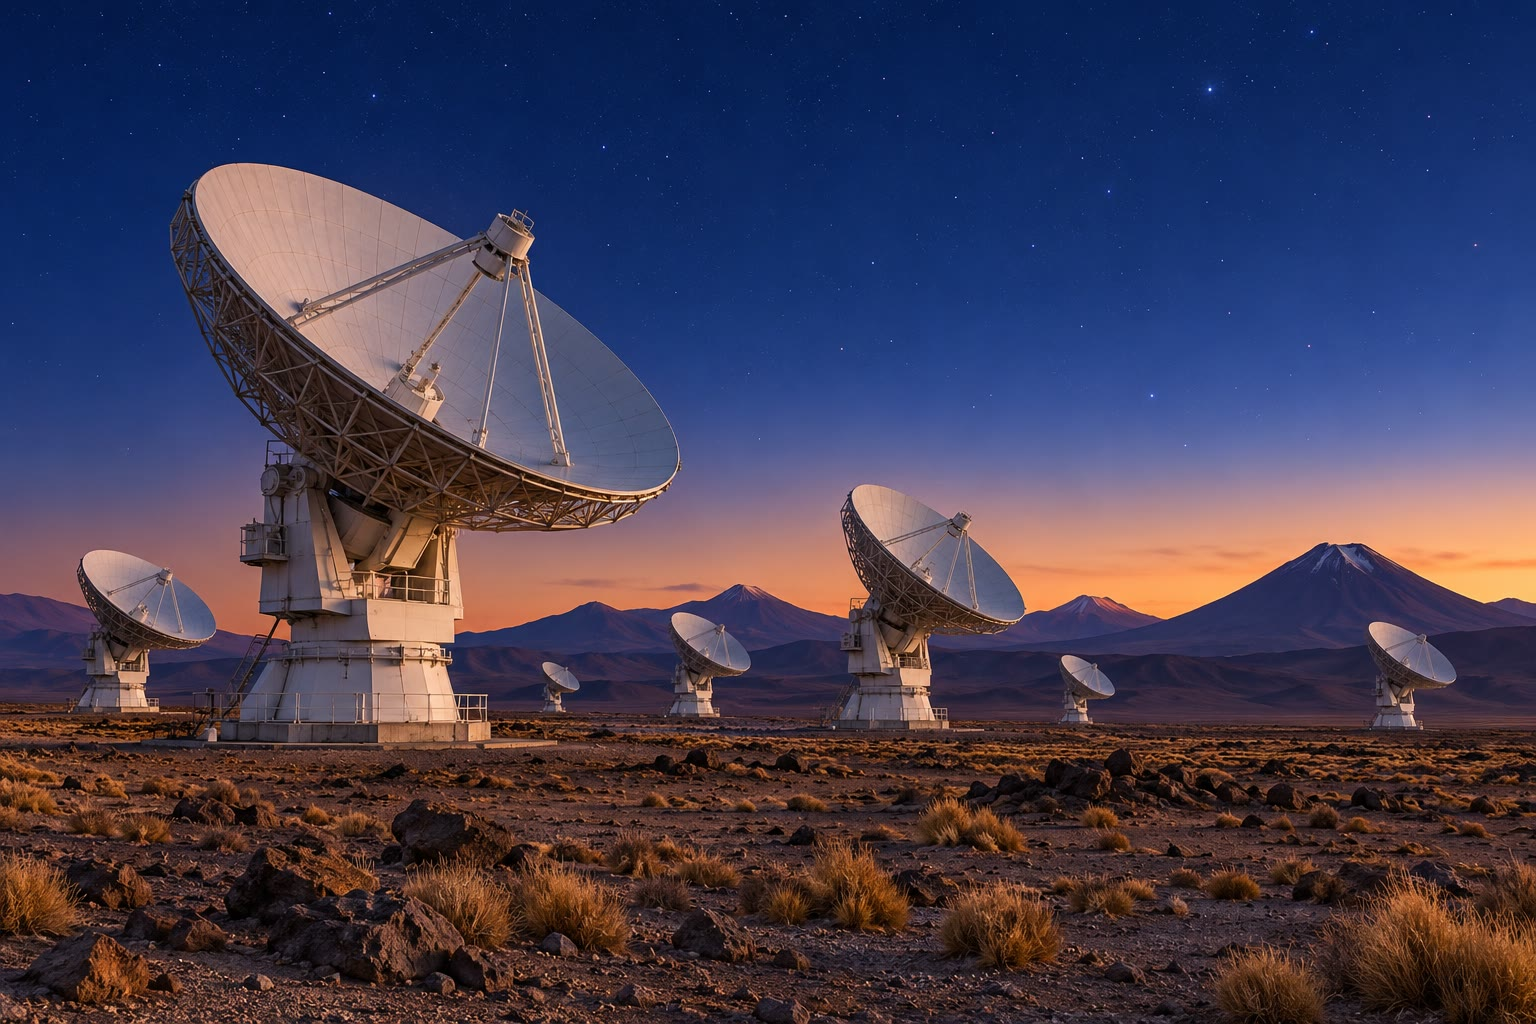
\includegraphics[width=\linewidth]{images/book4/ai/b2-radio-array.jpg}

{\scriptsize साँझ के समय एक ऊँचे मरुस्थलीय पठार पर रेडियो ऐंटेनाओं की एक पंक्ति
(AI से बनाया गया चित्रण)।}
\end{minipage}
% ledger: alma:hltau, alma:baselines
\end{inthelab}

\section{अभ्यास}

\begin{exercise}[$\star$]\label{exo:b2:ism-star-formation:1}
सूर्य के निकट माध्य अंतरतारकीय घनत्व \qty{2.7e-24}{g.cm^{-3}} है।
हाइड्रोजन परमाणु का द्रव्यमान \qty{1.67e-24}{g} लेकर प्रति घन सेंटीमीटर हाइड्रोजन
परमाणुओं की संख्या परिकलित कीजिए। उसकी तुलना \qty{101325}{Pa} और \qty{288}{K} पर
वायु में प्रति घन सेंटीमीटर अणुओं की संख्या से कीजिए ($n = P/k_{\mathrm B}T$)।
% ledger: ferriere:mean-density, const:kB
\end{exercise}

\begin{exercise}[$\star$]\label{exo:b2:ism-star-formation:2}
मान $M_J = 5.46$ सौर द्रव्यमान (\qty{10}{K} और प्रति घन सेंटीमीटर $10^4$ कणों पर)
और घनत्व के साथ $M_J$ के बदलने के नियम का उपयोग करके, \qty{10}{K} और प्रति घन सेंटीमीटर $10^2$
कणों पर \omterm{def:b2:ism-star-formation:jeans}{जीन्स द्रव्यमान} परिकलित कीजिए। \num{24000} सौर द्रव्यमान के वृषभ मेघ में कितने
\omterm{def:b2:ism-star-formation:jeans}{जीन्स द्रव्यमान} समाते हैं?
% ledger: goldsmith:taurus-mass
\end{exercise}

\begin{exercise}[$\star$]\label{exo:b2:ism-star-formation:3}
ध्वनि की समतापी चाल $c_s = (k_{\mathrm B}T/\mu m_u)^{1/2}$ को आणविक गैस
($\mu = 2.33$, $m_u = \qty{1.661e-27}{kg}$) के लिए \qty{10}{K} और \qty{100}{K} पर परिकलित कीजिए।
\qty{10}{K} पर एक ध्वनि-तरंग \qty{0.1}{pc} त्रिज्या के क्रोड को पार करने में
कितना समय लेती है, मिलियन वर्षों में?
% ledger: kauffmann:mu, nist:u, iau:parsec
\end{exercise}

\begin{exercise}[$\star$]\label{exo:b2:ism-star-formation:4}
प्रति घन सेंटीमीटर $10^5$ कणों वाले \omterm{def:b2:ism-star-formation:molecular-cloud}{सघन क्रोड} और $10^2$ वाले अदीप्त
मेघ का \omterm{def:b2:ism-star-formation:free-fall}{मुक्त पतन काल} परिकलित कीजिए ($\mu = 2.33$)। कौन अधिक तेज़ी से ढहता है,
और कितने गुना?
\end{exercise}

\begin{exercise}[$\star\star$]\label{exo:b2:ism-star-formation:5}
दिखाइए कि $M_J$ को $M_J = 5^{3/2}\,(3/4\pi)^{1/2}\,c_s^3\,G^{-3/2}\rho^{-1/2}$ लिखा जा सकता है।
स्थिर तापमान पर, किसी क्रोड का \omterm{def:b2:ism-star-formation:jeans}{जीन्स द्रव्यमान} आधा करने के लिए उसका घनत्व कितने गुना बढ़ना चाहिए?
स्थिर घनत्व पर, यदि क्रोड \qty{10}{K} से \qty{20}{K} तक गर्म हो जाए, तो
\omterm{def:b2:ism-star-formation:jeans}{जीन्स द्रव्यमान} कितने गुना बदलता है?
\end{exercise}

\begin{exercise}[$\star\star$]\label{exo:b2:ism-star-formation:6}
एक युवा तारे का द्रव्यमान सूर्य के बराबर है, त्रिज्या दोगुनी और ज्योति दोगुनी
($M_\odot = \qty{1.989e30}{kg}$, $R_\odot = \qty{6.96e8}{m}$,
$L_\odot = \qty{3.83e26}{W}$)। उसका केल्विन--हेल्महोल्ट्ज़ काल मिलियन वर्षों में
परिकलित कीजिए, और उसकी तुलना चक्रिकाओं की आयु से कीजिए।
% ledger: sun:mass, sun:R, sun:L
\end{exercise}

\begin{exercise}[$\star\star$]\label{exo:b2:ism-star-formation:7}
\qty{10}{K} के क्रोड में एक \omterm{def:b2:ism-star-formation:protostar}{आद्यतारे} की अभिवृद्धि-दर $c_s^3/G$ प्रति वर्ष सौर द्रव्यमान में
परिकलित कीजिए, और एक सौर द्रव्यमान जुटाने में लगने वाला समय भी। यही
प्रश्न \qty{20}{K} के क्रोड के लिए हल कीजिए।
\end{exercise}

\begin{exercise}[$\star\star$]\label{exo:b2:ism-star-formation:8}
\cref{prop:b2:ism-star-formation:grain} और $L_\odot = \qty{3.83e26}{W}$ से,
सूर्य से वह दूरी खगोलीय इकाइयों में परिकलित कीजिए जिस पर एक कण
\qty{1300}{K} तक पहुँचता है, जो उस तापमान के निकट है जिस पर सामान्य सिलिकेट
संघनित होते हैं (\cref{ch:b2:planet-formation-meteorites}), और
बृहस्पति की दूरी, \qty{5.2}{au}, पर एक कण का तापमान भी।
% ledger: sun:L, const:sigma, const:au
\end{exercise}

\begin{exercise}[$\star\star$]\label{exo:b2:ism-star-formation:9}
एचएल टॉरी की चक्रिका की गैस लगभग \num{1.3} सौर द्रव्यमान के तारे के चारों ओर
घूमती है। \qty{100}{au} पर केप्लरीय चाल और कक्षीय आवर्तकाल परिकलित कीजिए।
यदि तंत्र एक मिलियन वर्ष पुराना है, तो तारे के बनने के बाद से \qty{100}{au} पर स्थित
गैस ने कितने चक्कर लगाए हैं?
% ledger: alma:hltau
\end{exercise}

\begin{exercise}[$\star\star\star$]\label{exo:b2:ism-star-formation:10}
त्रिज्या $R$ के उस गोले की गुरुत्वीय ऊर्जा ज्ञात कीजिए जिसमें घनत्व
$\rho(r) = \rho_0 R/r$ के अनुसार घटता है, और उसकी तुलना समान द्रव्यमान और त्रिज्या के
एकसमान गोले की ऊर्जा से कीजिए। क्या द्रव्यमान को केंद्र की ओर सांद्रित करने से
मेघ को उसकी तापीय ऊर्जा से थामे रखना आसान होता है या कठिन?
\end{exercise}

\begin{exercise}[$\star\star\star$]\label{exo:b2:ism-star-formation:11}
\qty{0.1}{pc} त्रिज्या का एक क्रोड कोणीय चाल
$\Omega = \qty{1e-14}{rad.s^{-1}}$ से दृढ़ पिंड की भाँति घूमता है। उसका घूर्णन-आवर्तकाल, उसके
विषुवत पर गैस का विशिष्ट कोणीय संवेग $j = \Omega R^2$, और एक सौर द्रव्यमान के तारे के चारों ओर उस
गैस की अपकेंद्री त्रिज्या खगोलीय इकाइयों में परिकलित कीजिए।
क्रोड के भीतर से आने वाली गैस तारे के अधिक निकट क्यों उतरती है?
\end{exercise}

\begin{exercise}[$\star\star\star$]\label{exo:b2:ism-star-formation:12}
पिछले अनुभाग के चित्र के पाँच सबसे युवा तारागुच्छों के चक्रिका-अंश
0.3, 1.5, 2.3, 3.2 और \qty{5.0}{Myr} पर क्रमशः $0.85$, $0.80$, $0.65$, $0.52$ और $0.12$ हैं।
हाथ से न्यूनतम-वर्ग सरल रेखा $f = a - bt$ बिठाइए
(पहले माध्य, फिर $\sum(t - \bar t)(f - \bar f)$ और
$\sum(t - \bar t)^2$ परिकलित कीजिए)। वह किस आयु पर आधे तक, और किस आयु पर शून्य तक पहुँचती है? उस आयु के बाद
सरल रेखा एक कमज़ोर मॉडल क्यों है?
% ledger: haisch:disc-fractions
\end{exercise}

\section{समस्या: आल्ड्रा मेघ का एक क्रोड}

\begin{problem}[{सप्ताहांत समस्या --- धूल-मानचित्र से पढ़े गए एक सघन क्रोड का द्रव्यमान और
स्थायित्व, उसके आद्यतारे का जन्म और उसकी चक्रिका का आकार}]
\label{pb:b2:ism-star-formation:1}
% values: calc/ch01.py
% ledger: kauffmann:mu, nist:u, iau:parsec, const:G, const:kB, sun:mass, sun:R, sun:L, const:au, const:sigma, bt07:cores, alma:hltau
आल्ड्रा मेघ एक कल्पित अदीप्त मेघ है। उसकी धूल का मिलीमीटर मानचित्र
\qty{0.08}{pc} त्रिज्या का एक गोल क्रोड दिखाता है, जिसका माध्य स्तंभ-घनत्व
प्रति वर्ग सेंटीमीटर $N(\ce{H2}) = \num{1.5e22}$ हाइड्रोजन अणु है।
अमोनिया की एक रेखा से गैस का तापमान, \qty{10}{K}, और क्रोड के आर-पार प्रति पारसेक
\qty{0.4}{km.s^{-1}} की वेग-प्रवणता मिलती है, जिसे दृढ़ पिंड के
घूर्णन के रूप में पढ़ा जाता है। $G = \qty{6.674e-11}{m^3.kg^{-1}.s^{-2}}$,
$k_{\mathrm B} = \qty{1.381e-23}{J.K^{-1}}$, $m_u = \qty{1.661e-27}{kg}$,
\qty{1}{pc} $= \qty{3.086e16}{m}$, \qty{1}{au} $= \qty{1.496e11}{m}$, एक वर्ष
\qty{3.156e7}{s}, $M_\odot = \qty{1.989e30}{kg}$, $R_\odot = \qty{6.96e8}{m}$,
$L_\odot = \qty{3.83e26}{W}$, $\sigma = \qty{5.67e-8}{W.m^{-2}.K^{-4}}$ लीजिए; हीलियम सहित
प्रति हाइड्रोजन अणु द्रव्यमान $2.8\,m_u$ है, और प्रति कण माध्य द्रव्यमान
$2.33\,m_u$।

\medskip
\noindent\textbf{भाग I --- द्रव्यमान और घनत्व।}
\begin{enumerate}
  \item क्रोड की त्रिज्या को मीटर में बदलिए।
  \item स्तंभ का प्रति वर्ग मीटर द्रव्यमान, $2.8\,m_u N$, परिकलित कीजिए।
  \item क्रोड का द्रव्यमान किलोग्राम में और सौर द्रव्यमान में निकालिए।
  \item उसका आयतन और उसका माध्य घनत्व परिकलित कीजिए।
  \item प्रति घन सेंटीमीटर कणों की संख्या परिकलित कीजिए।
  \item क्या यह दूसरे अनुभाग की तालिका के अर्थ में एक \omterm{def:b2:ism-star-formation:molecular-cloud}{सघन क्रोड} है?
\end{enumerate}

\noindent\textbf{भाग II --- स्थायित्व।}
\begin{enumerate}[resume]
  \item क्रोड की गैस का \omterm{def:b2:ism-star-formation:jeans}{जीन्स द्रव्यमान} सौर द्रव्यमान में परिकलित कीजिए।
  \item क्रोड में कितने \omterm{def:b2:ism-star-formation:jeans}{जीन्स द्रव्यमान} हैं? क्या वह स्थायी है?
  \item \omterm{def:b2:ism-star-formation:jeans}{जीन्स लंबाई} परिकलित कीजिए और उसकी तुलना क्रोड की त्रिज्या से कीजिए।
  \item यदि गैस \qty{20}{K} पर होती तो \omterm{def:b2:ism-star-formation:jeans}{जीन्स द्रव्यमान} क्या होता? क्या तब भी
        क्रोड ढहता?
  \item क्रोड का \omterm{def:b2:ism-star-formation:free-fall}{मुक्त पतन काल} हज़ार वर्षों में परिकलित कीजिए।
  \item उसकी तुलना उस समय से कीजिए जो एक ध्वनि-तरंग क्रोड को पार करने में लेती है। कौन-सी
        प्रक्रिया अधिक तेज़ है, और उसका क्या अर्थ है?
\end{enumerate}

\noindent\textbf{भाग III --- आद्यतारा।}
\begin{enumerate}[resume]
  \item क्रोड में ध्वनि की चाल परिकलित कीजिए।
  \item अभिवृद्धि-दर $c_s^3/G$ प्रति वर्ष सौर द्रव्यमान में परिकलित कीजिए।
  \item इस दर पर एक सौर द्रव्यमान जुटाने में लगने वाला समय परिकलित कीजिए।
  \item यदि क्रोड का एक-तिहाई भाग तारों में बदलता है, तो वह एक सौर द्रव्यमान के
        कितने तारे बना सकता है?
  \item आवरण के समाप्त होने पर तारे का द्रव्यमान एक सौर द्रव्यमान, त्रिज्या तीन सौर
        त्रिज्याएँ और ज्योति चार सौर ज्योतियाँ है। उसका केल्विन--हेल्महोल्ट्ज़ काल परिकलित कीजिए।
  \item क्या वह अभिवृद्धि-काल से लंबा है या छोटा? तब वह किस प्रकार का
        तारा है?
\end{enumerate}

\noindent\textbf{भाग IV --- चक्रिका।}
\begin{enumerate}[resume]
  \item वेग-प्रवणता को कोणीय चाल $\Omega$ में,
        \unit{rad.s^{-1}} में, बदलिए।
  \item क्रोड के विषुवत पर गैस का विशिष्ट कोणीय संवेग $j = \Omega R^2$
        परिकलित कीजिए।
  \item एक सौर द्रव्यमान के तारे के चारों ओर उसकी अपकेंद्री त्रिज्या खगोलीय
        इकाइयों में परिकलित कीजिए।
  \item एक सौर ज्योति वाले तारे से \qty{1}{au} और \qty{30}{au} पर
        एक कण का तापमान परिकलित कीजिए।
  \item यदि जल-बर्फ़ \qty{180}{K} से नीचे बची रहती है, तो इस चक्रिका की
        हिम रेखा कहाँ है?
  \item प्रश्न 15 के तारे को जुटाने में लगने वाला समय, इस समस्या की मुख्य
        संख्या, हज़ार वर्षों में बताइए, और उसकी तुलना
        प्रश्न 11 के \omterm{def:b2:ism-star-formation:free-fall}{मुक्त पतन काल} से कीजिए।
\end{enumerate}
\end{problem}
